\documentclass[border=5mm]{standalone}
\usepackage{amsmath}
\usepackage{amssymb}
\usepackage{array}
\usepackage{booktabs}
\usepackage{tikz}
\usetikzlibrary{shapes.geometric, arrows.meta, positioning, fit, backgrounds}

\definecolor{stepblue}{RGB}{100,150,200}
\definecolor{stepgreen}{RGB}{120,180,120}
\definecolor{steporange}{RGB}{230,150,80}

\begin{document}

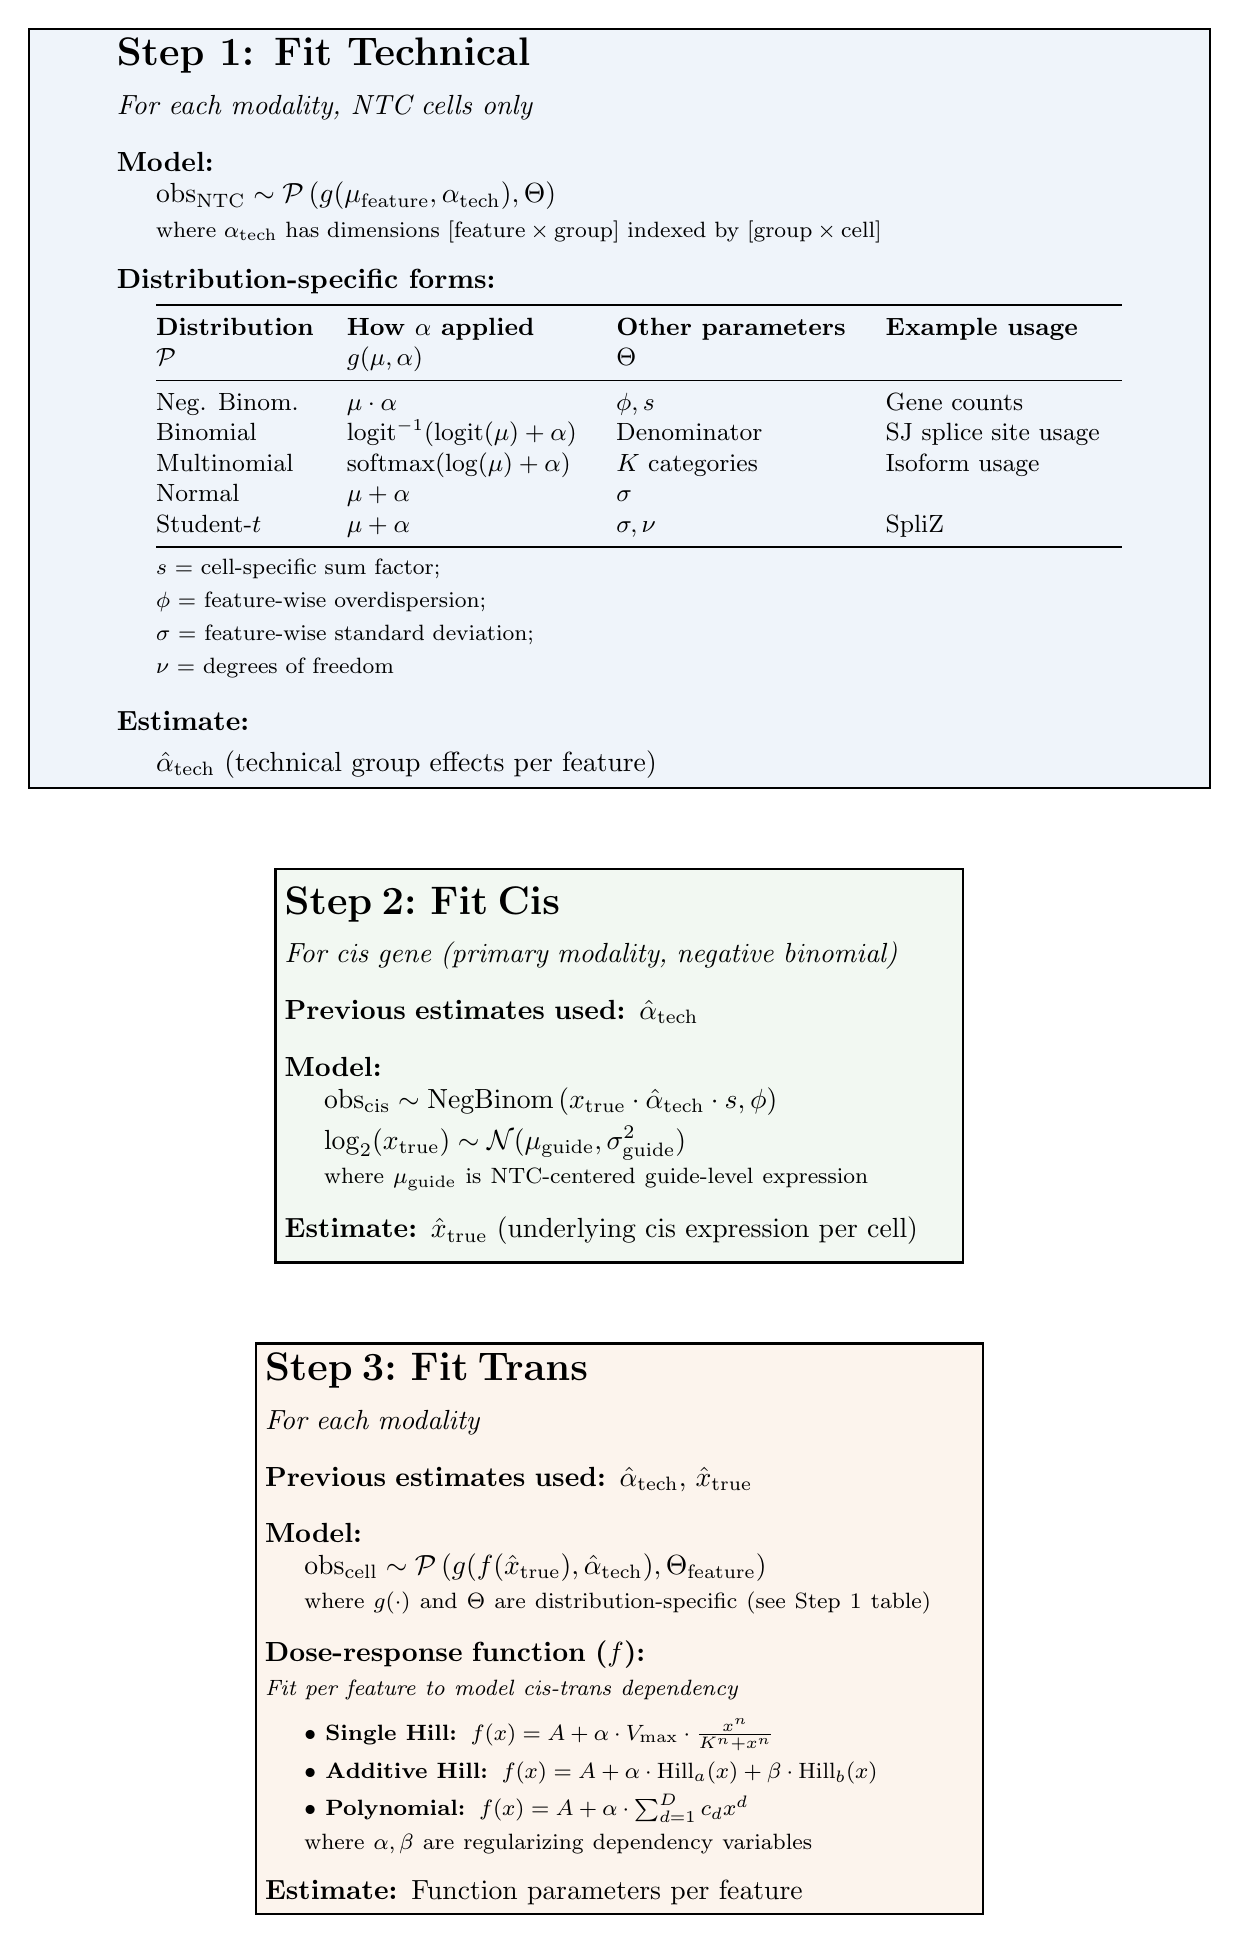
\begin{tikzpicture}[
  node distance=1cm,
  box/.style={rectangle, draw, thick, minimum width=11cm, align=left}
]

% Step 1: Fit Technical
\node[box, fill=stepblue!10, minimum width=15cm, minimum height=8cm] (step1) {
  \textbf{\Large Step 1: Fit Technical} \\[0.2cm]
  \textit{For each modality, NTC cells only} \\[0.3cm]

  \textbf{Model:} \\[0.1cm]
  \hspace{0.5cm}\parbox{10cm}{%
  $\displaystyle
  \text{obs}_{\text{NTC}} \sim \mathcal{P}\left(g(\mu_{\text{feature}}, \alpha_{\text{tech}}), \Theta\right)
$ \\[0.1cm]
  \footnotesize where $\alpha_{\text{tech}}$ has dimensions $[\text{feature} \times \text{group}]$ indexed by $[\text{group} \times \text{cell}]$
  } \\[0.3cm]

  \normalsize
  \textbf{Distribution-specific forms:} \\[0.1cm]
  \hspace{0.5cm}\small
  \begin{tabular}{@{}p{2cm} p{3cm} p{3cm} p{3cm}@{}}
    \toprule
    \textbf{Distribution} & \textbf{How $\alpha$ applied} & \textbf{Other parameters} & \textbf{Example usage} \\
    \textbf{$\mathcal{P}$} & \textbf{$g(\mu, \alpha)$} & \textbf{$\Theta$} & \\
    \midrule
    Neg. Binom. & $\mu \cdot \alpha$ & $\phi, s$ & Gene counts \\
    Binomial & logit$^{-1}($logit$(\mu) + \alpha)$ & Denominator & SJ splice site usage \\
    Multinomial & softmax(log$(\mu) + \alpha)$ & $K$ categories & Isoform usage \\
    Normal & $\mu + \alpha$ & $\sigma$ & \\
    Student-$t$ & $\mu + \alpha$ & $\sigma, \nu$ & SpliZ \\
    \bottomrule
  \end{tabular} \\[0.1cm]
  \hspace{0.5cm}\footnotesize $s$ = cell-specific sum factor;\\
  \hspace{0.5cm}\footnotesize $\phi$ = feature-wise overdispersion;\\
  \hspace{0.5cm}\footnotesize $\sigma$ = feature-wise standard deviation;\\
  \hspace{0.5cm}\footnotesize $\nu$ = degrees of freedom \\[0.3cm]

  \normalsize
  \textbf{Estimate:} \\[0.1cm]
  \hspace{0.5cm}$\hat{\alpha}_{\text{tech}}$ (technical group effects per feature)
};

% Step 2: Fit Cis
\node[rectangle, draw, thick, fill=stepgreen!10, below=of step1, align=left, text width=8.5cm, minimum height=5cm] (step2) {
  \textbf{\Large Step 2: Fit Cis} \\[0.2cm]
  \textit{For cis gene (primary modality, negative binomial)} \\[0.3cm]

  \textbf{Previous estimates used:} $\hat{\alpha}_{\text{tech}}$ \\[0.3cm]

  \textbf{Model:} \\[0.1cm]
  \hspace{0.5cm}\parbox{7.5cm}{%
  $\displaystyle
  \text{obs}_{\text{cis}} \sim \text{NegBinom}\left(x_{\text{true}} \cdot \hat{\alpha}_{\text{tech}} \cdot s, \phi\right) $ \\[0.1cm]
  $\displaystyle
  \log_2(x_{\text{true}}) \sim \mathcal{N}(\mu_{\text{guide}}, \sigma_{\text{guide}}^2)  $ \\[0.1cm]
  \footnotesize where $\mu_{\text{guide}}$ is NTC-centered guide-level expression
  } \\[0.3cm]

  \normalsize
  \textbf{Estimate:} $\hat{x}_{\text{true}}$ (underlying cis expression per cell)
};

% Step 3: Fit Trans
\node[rectangle, draw, thick, fill=steporange!10, below=of step2, align=left, text width=9cm, minimum height=7cm] (step3) {
  \textbf{\Large Step 3: Fit Trans} \\[0.2cm]
  \textit{For each modality} \\[0.3cm]

  \textbf{Previous estimates used:} $\hat{\alpha}_{\text{tech}}$, $\hat{x}_{\text{true}}$ \\[0.3cm]

  \textbf{Model:} \\[0.1cm]
  \hspace{0.5cm}\parbox{8cm}{%
  $\displaystyle
  \text{obs}_{\text{cell}} \sim \mathcal{P}\left( g(f(\hat{x}_{\text{true}}), \hat{\alpha}_{\text{tech}}), \Theta_{\text{feature}}\right)
$ \\[0.1cm]
  \footnotesize where $g(\cdot)$ and $\Theta$ are distribution-specific (see Step 1 table)
  } \\[0.3cm]

  \normalsize
  \textbf{Dose-response function ($f$):} \\[0.1cm]
  \footnotesize \textit{Fit per feature to model cis-trans dependency} \\[0.2cm]
  \hspace{0.5cm}\parbox{8cm}{%
  $\bullet$ \textbf{Single Hill:} $f(x) = A + \alpha \cdot V_{\max} \cdot \frac{x^n}{K^n + x^n}$ \\[0.1cm]
  $\bullet$ \textbf{Additive Hill:} $f(x) = A + \alpha \cdot \text{Hill}_a(x) + \beta \cdot \text{Hill}_b(x)$ \\[0.1cm]
  $\bullet$ \textbf{Polynomial:} $f(x) = A + \alpha \cdot \sum_{d=1}^{D} c_d x^d$ \\[0.1cm]
  \footnotesize where $\alpha, \beta$ are regularizing dependency variables
  } \\[0.3cm]

  \normalsize
  \textbf{Estimate:} Function parameters per feature
};


\end{tikzpicture}

\end{document}
